\chapter{Юридично-документальний рівень}

\section{Вступ}

Відповідно до фреймворку системи, верхній п'ятий рівень визначає BPMN-процеси, згідно з якими здійснюється точне відображення юридичних відносин у вигляді електронного документообігу. Кожен крок такого процесу та всі супровідні документи підписуються особистим ключем КЕП (кваліфікованого електронного підпису) посадової особи. Це створює надійне підґрунтя для проведення аудитів, диспутів та службових розслідувань Міністерством юстиції України, із залученням власного Засвідчувального центру в просторі інтернет-імен. Окрім того, цей рівень системи повністю орієнтований на аналітику та прозору взаємодію з громадянами через Систему електронної взаємодії органів виконавчої влади (СЕВ ОВВ).

Юридично-документальні системи класу ERP/1 будуються на базі надійного сховища з єдиним простором ключів (на кшталт Facebook RocksDB), що здатне працювати через інтерфейси Intel SPDK на швидкісних NVMe дисках, наприклад, у складі таких кластерних сховищ, як CEPH. Архітектура враховує той факт, що обсяг обігу документів на великих державних чи комерційних підприємствах може сягати 1 ТБ на рік.

\subsection{Види документообігів}

\subsubsection{Постанова №55 КМУ}
\subsubsection{Наказ №124 МОУ}
\subsubsection{Закупівлі}
\subsubsection{Провадження}
\subsubsection{Зброя}

\subsection{Функціональні можливості}

\newpage
\section{Модулі підприємства}

ERP/1 є потужним комплексом інструментальних бібліотек (N2O.DEV) та підсистем додатків (ERP.UNO), який використовує загальну шину повідомлень і спільну розподілену базу даних для побудови швидкісних операційних вітрин.
\\
\\
\textbf{ERP} — Даний модуль обліково-реєстраційного рівня надійно зберігає основну ієрархічну структуру підприємства, її схему, метаінформацію про базові типи даних, а також безпосередньо саму інформацію: записи про персонал, інвентар, компанії-контрагенти та офіси підприємства.
\\
\\
\textbf{CRM} — Система функціонального управління зв'язками з громадськістю та органами виконавчої влади: являє собою базову вітально необхідну реалізацію вимог постанови №55 КМУ.
\\
\\
\textbf{CART} — Система гнучкого управління реєстрами: являє собою реалізацію надійного базового сервера для виконання широкого спектра реєстрових та класифікаторних задач.

\newpage
\section{Управління ресурсами}

Головним чином інформаційна інфраструктура підприємства складається з активних обчислювальних ресурсів (додатків та сервісів, запущених у шині) та пасивних накопичувальних ресурсів (даних, збережених у розподіленій базі).
\\
\\
Для ефективного управління обчислювальними ресурсами SOA-архітектура як системна модель пропонує асинхронний протокол віддаленого виклику процедур безпосередньо на шинах. Разом з екосистемою N2O можна використовувати MQTT та інші транспортабельні шини, послуговуючись такими протоколами, як TCP та WebSocket. Ці асинхронні комунікації часто називають протоколами реального часу, оскільки функції відправлення повідомлень у них завжди миттєво повертають результат (fire-and-forget). Що ж стосується протоколів для традиційної публікації та доступу до даних, то у цьому контексті може виявитися особливо доречним застосування класичного синхронного протоколу HTTP.

\newpage
\section{Архітектура врядувальних CRM-систем}

\subsection{Сторінки}

Нижче наведено базовий перелік маршрутів сторінок:

\begin{lstlisting}
def route(<<"ldap", _::binary>>), do: LDAP.Index
def route(<<"crm",  _::binary>>), do: CRM.Index
def route(<<"rmk",  _::binary>>), do: RMK.Index
def route(<<"kvs",  _::binary>>), do: KVS.Index
def route(<<"act",  _::binary>>), do: BPE.Actor
def route(<<"help", _::binary>>), do: HELP.Index
\end{lstlisting}

\subsubsection{LDAP}

Сторінка безпечної авторизації та ідентифікації користувачів.

\begin{figure}[!htbp]
\centerline{\includegraphics[scale=0.25]{LDAP.PNG}}
\caption{Сторінка авторизації}
\end{figure}

\subsection{Комболукап}
\subsection{Сервіси}
\subsection{СЕВ ОВВ}
\subsection{Шаблони}
\subsection{Дерева}

\newpage
\subsection{Процеси}

Даний керівний модуль надійно інкапсулює визначення сутностей Схеми, Бізнес-процесів та Форм, які безперервно використовуються у системі Infotech-ERP згідно з академічною методологією фреймворку Закмана.

\subsubsection{Формування нормативно-довідкової інформації}

У цьому модулі автоматизації виділяються такі основні типи процесів для організаційно-розпорядчих документів: «Накази», «Протоколи», «Доручення керівництва».

\subsubsection{Обробка вхідних документів}

Усі вхідні документи автоматично надходять в УДСД (Управління документального забезпечення), ВОРЗГ (Відділ організації роботи зі зверненнями громадян) та ВОДПІ. При надходженні документа уповноважена посадова особа зазначених структурних підрозділів сумлінно реєструє його в системі, після чого стартує процес його подальшої маршрутизації та обробки.

\begin{figure}[!htbp]
\centerline{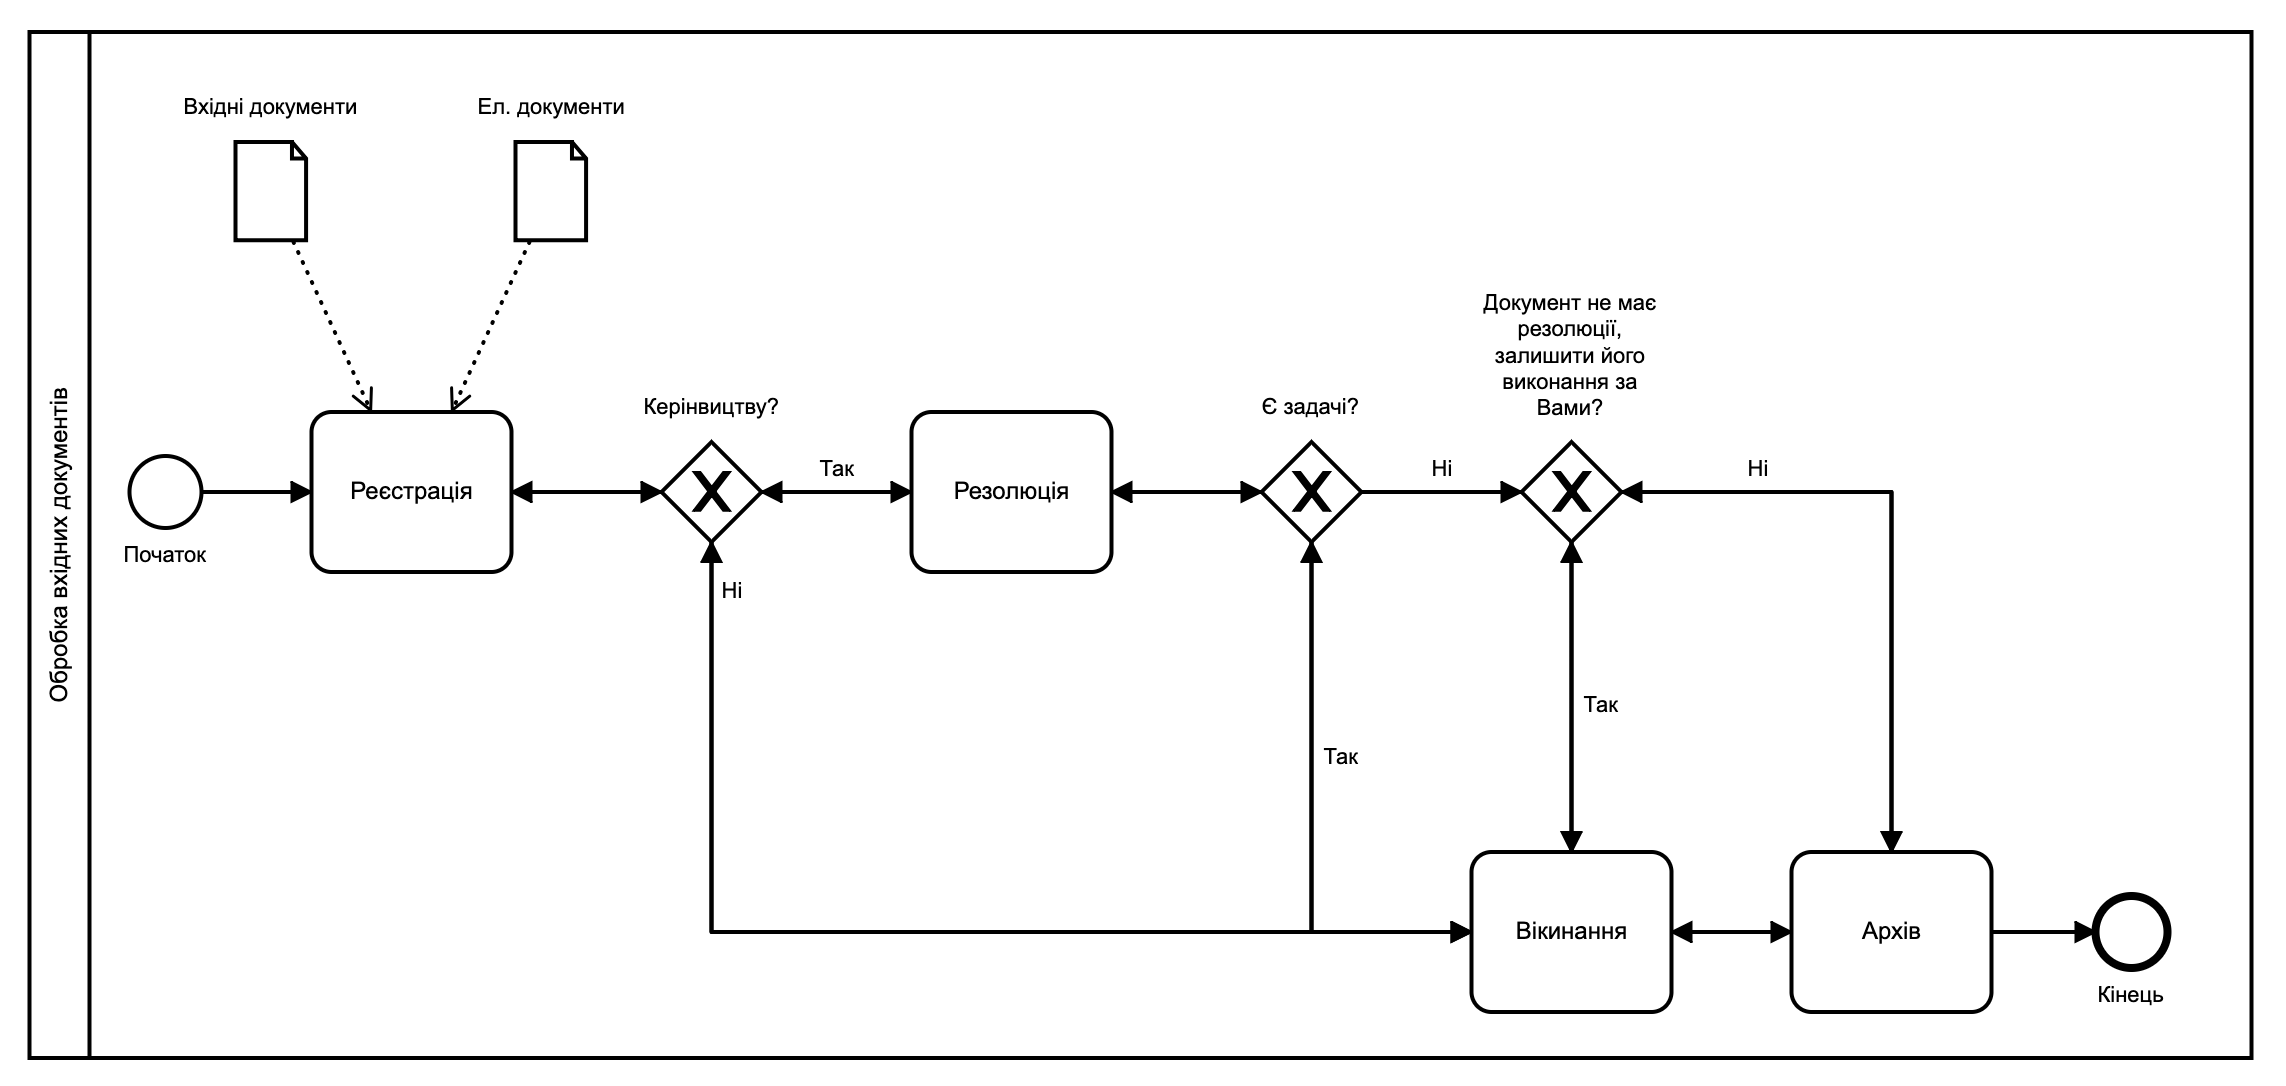
\includegraphics[scale=0.25]{handleInputDoc.png}}
\caption{Бізнес-процес обробки вхідних документів}
\end{figure}

Далі зареєстрований вхідний документ надходить або Міністру, Заступнику міністра, чи Державному секретарю для накладання управлінської резолюції, або безпосередньо спрямовується до профільного структурного підрозділу на виконання.

\subsubsection{Вхідні документи}

\begin{figure}[!htbp]
\centerline{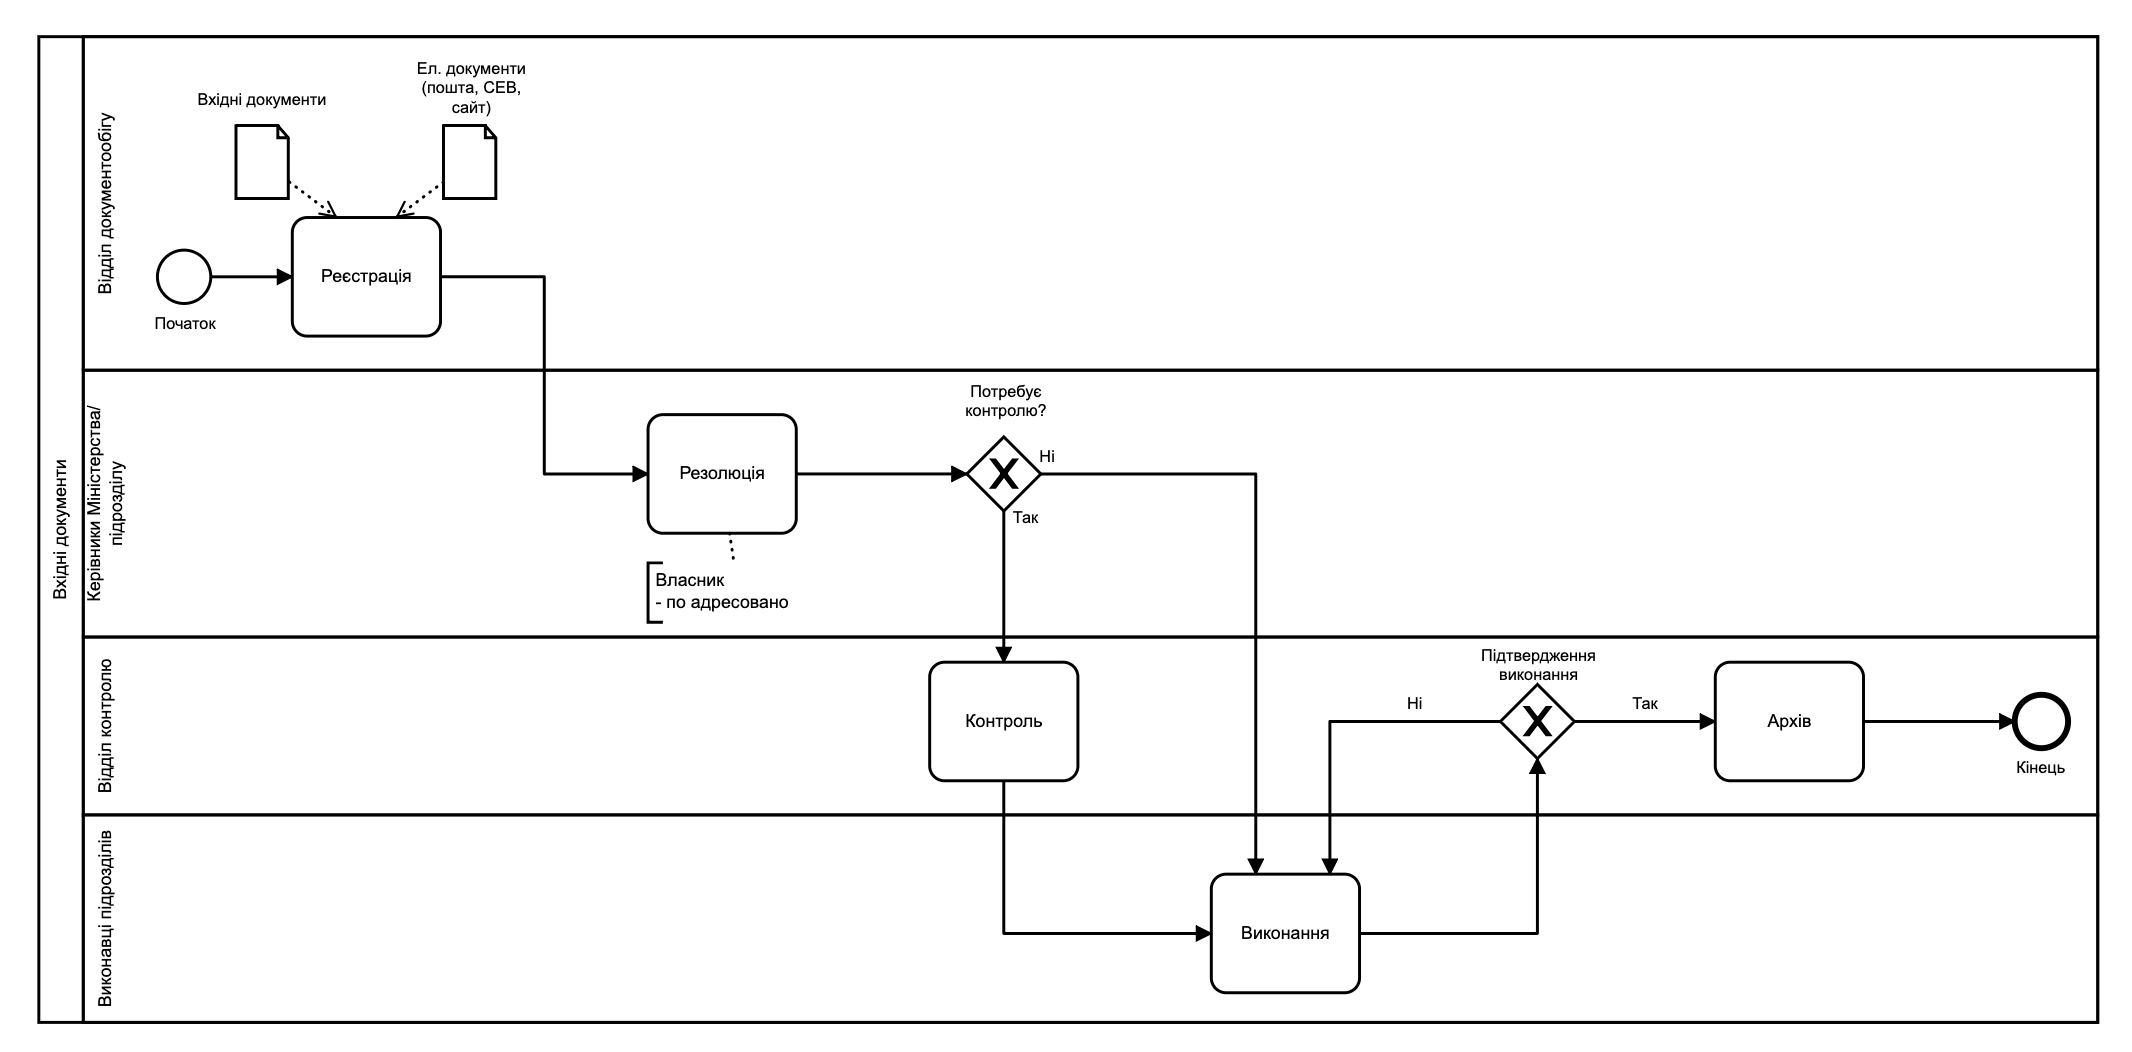
\includegraphics[scale=0.27]{inputDoc.png}}
\caption{Бізнес-процес обробки вхідних документів}
\end{figure}

\subsubsection{Вихідні документи}

\begin{figure}[!htbp]
\centerline{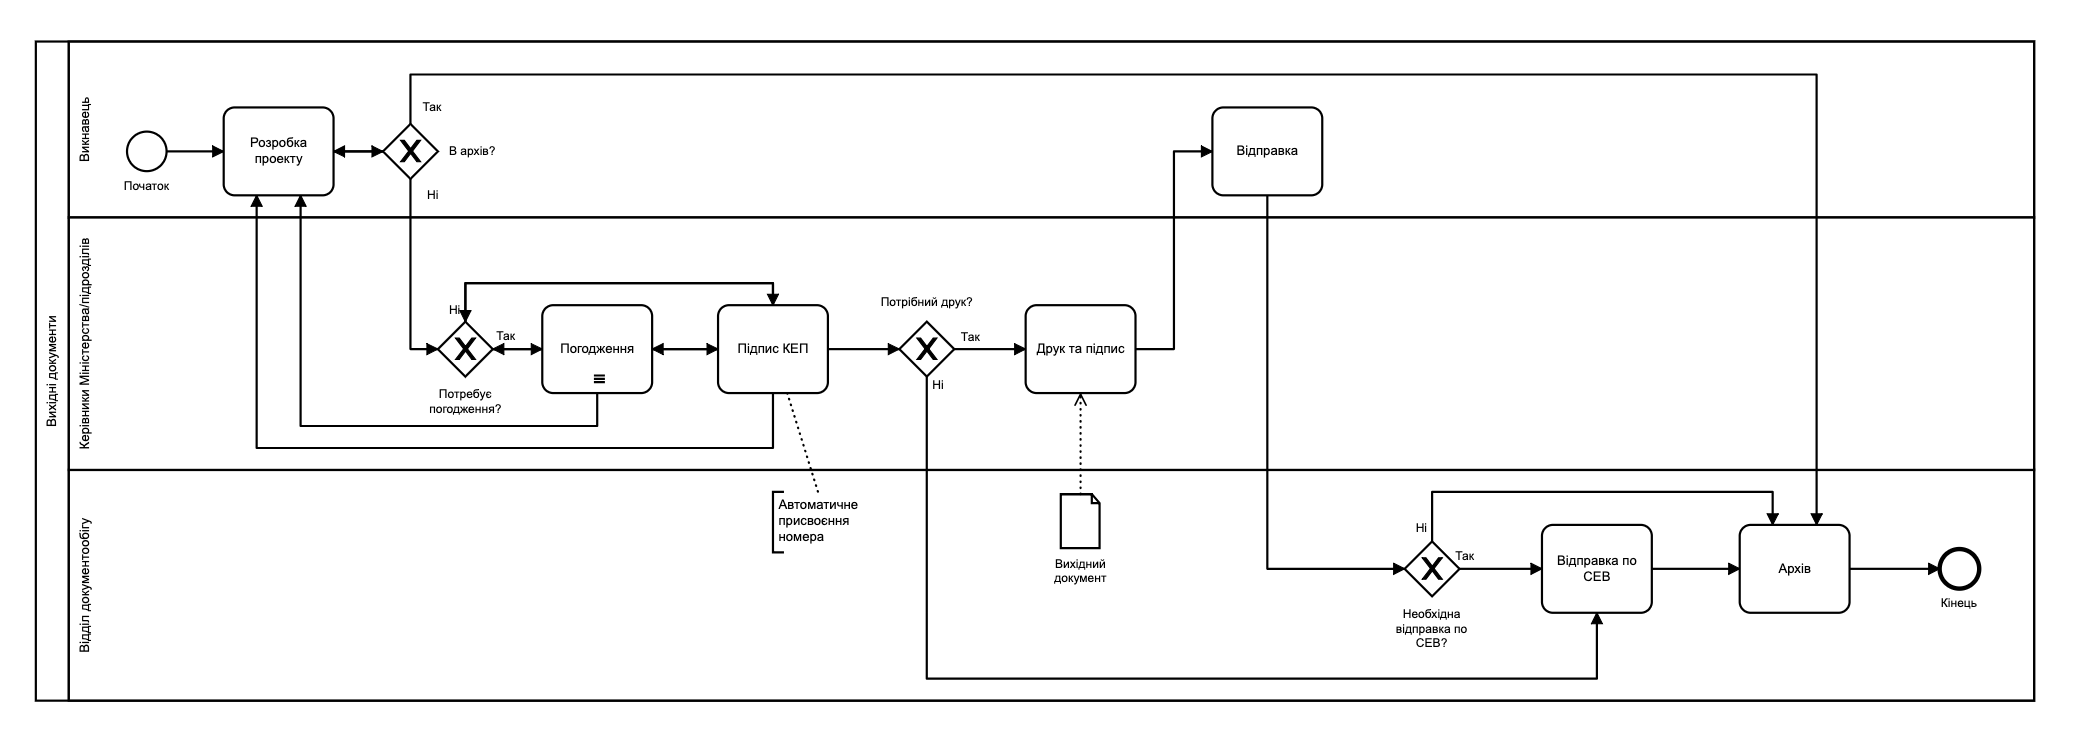
\includegraphics[scale=0.27]{outputDoc.png}}
\caption{Бізнес-процес підготовки вихідних документів}
\end{figure}

Вихідні документи формуються та створюються безпосередньо в підрозділах, які виступають ініціаторами документа. Вони можуть виникати як з власної ініціативи співробітників Міністерства, так і як прямий результат або відповідь на обробку вхідних документів. Якщо вихідний документ логічно пов'язаний із вхідним документом, то відповідальному працівнику система рекомендує обов'язково вказати семантичне посилання на пов'язаний документ-першоджерело. Регламентна обробка документів виконується за єдиним еталонним уніфікованим бізнес-процесом, незалежно від конкретного місця виникнення документа. Від початку в системі реєструється проект вихідного документа, який неодмінно повинен бути завізований і погоджений із визначеним кваліфікованим переліком погоджуючих посадових осіб. Щойно фінальний підписант накладає свій КЕП, документу автоматично присвоюється вихідний реєстраційний номер, і система ініціює його відправку.

\subsubsection{Внутрішні документи}

Внутрішні документи можуть створюватися та вводитися всіма авторизованими учасниками контуру документообігу. Серед них виділяються такі основні стандартизовані бізнес-процеси внутрішніх документів: «Доповідна записка», «Службовий лист».

\begin{figure}[!htbp]
\centerline{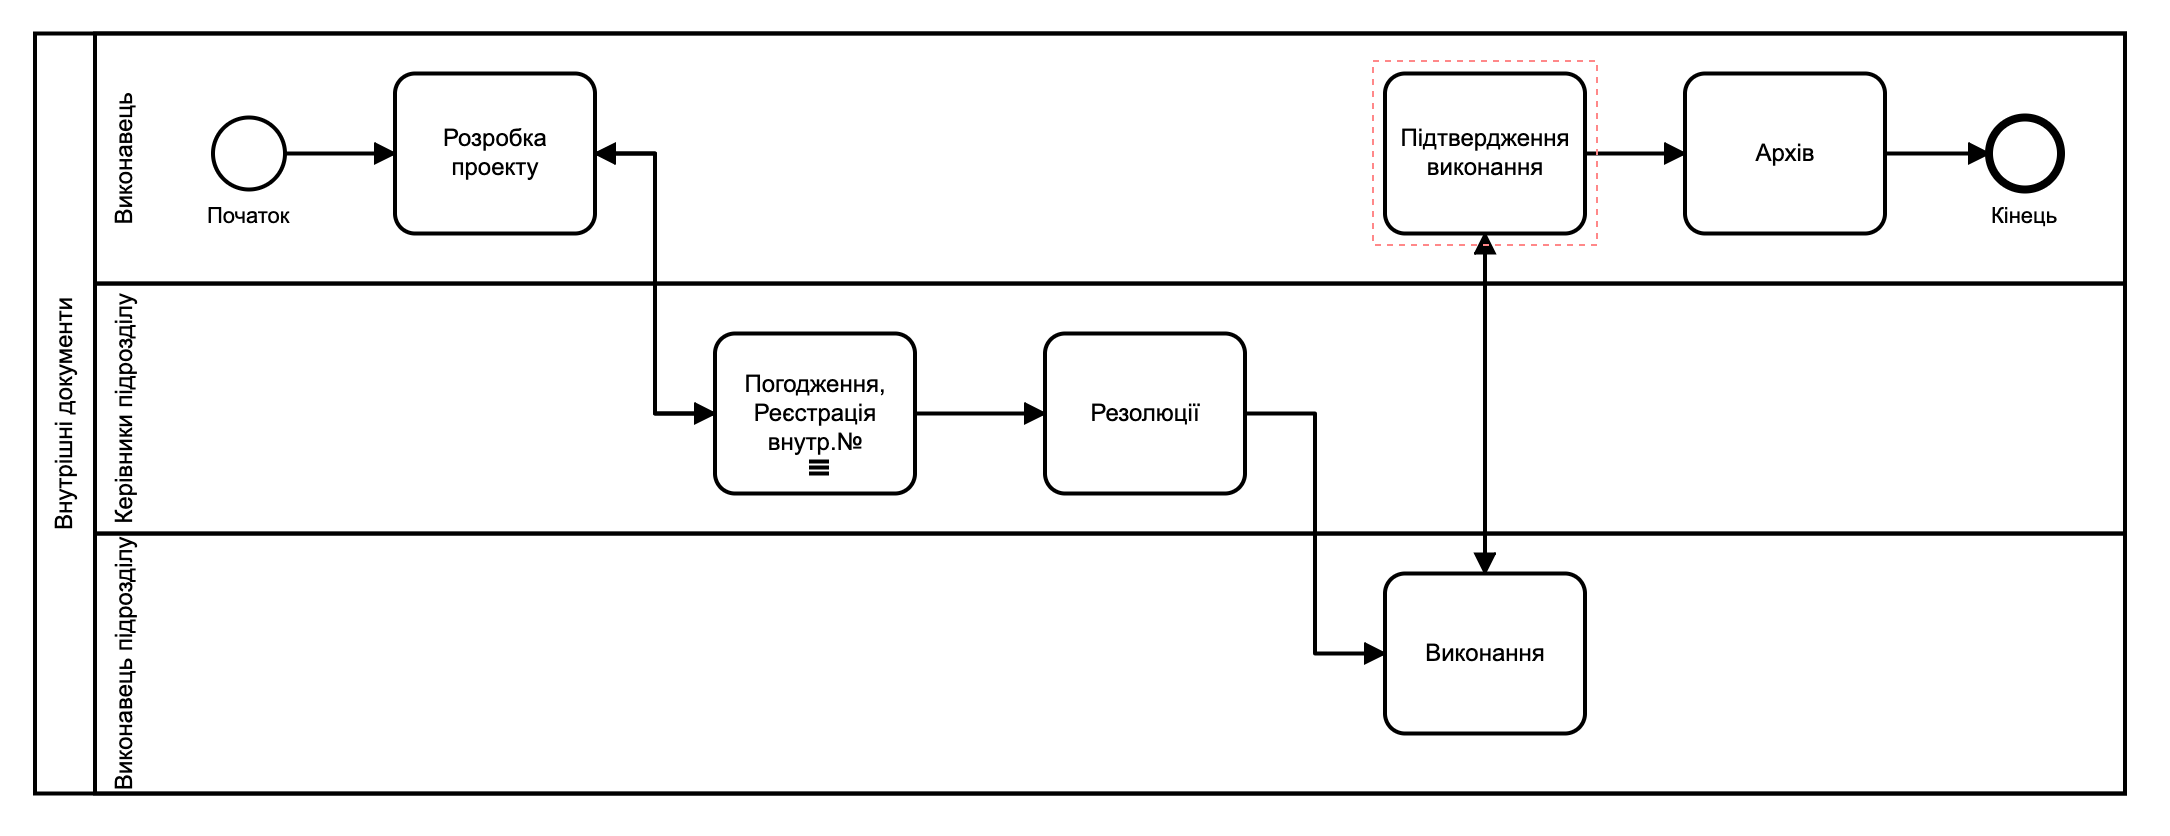
\includegraphics[scale=0.27]{internalDoc.png}}
\caption{Бізнес-процес обігу внутрішніх документів}
\end{figure}

\subsubsection{Організаційно-розпорядчі документи}

\begin{figure}[!htbp]
\centerline{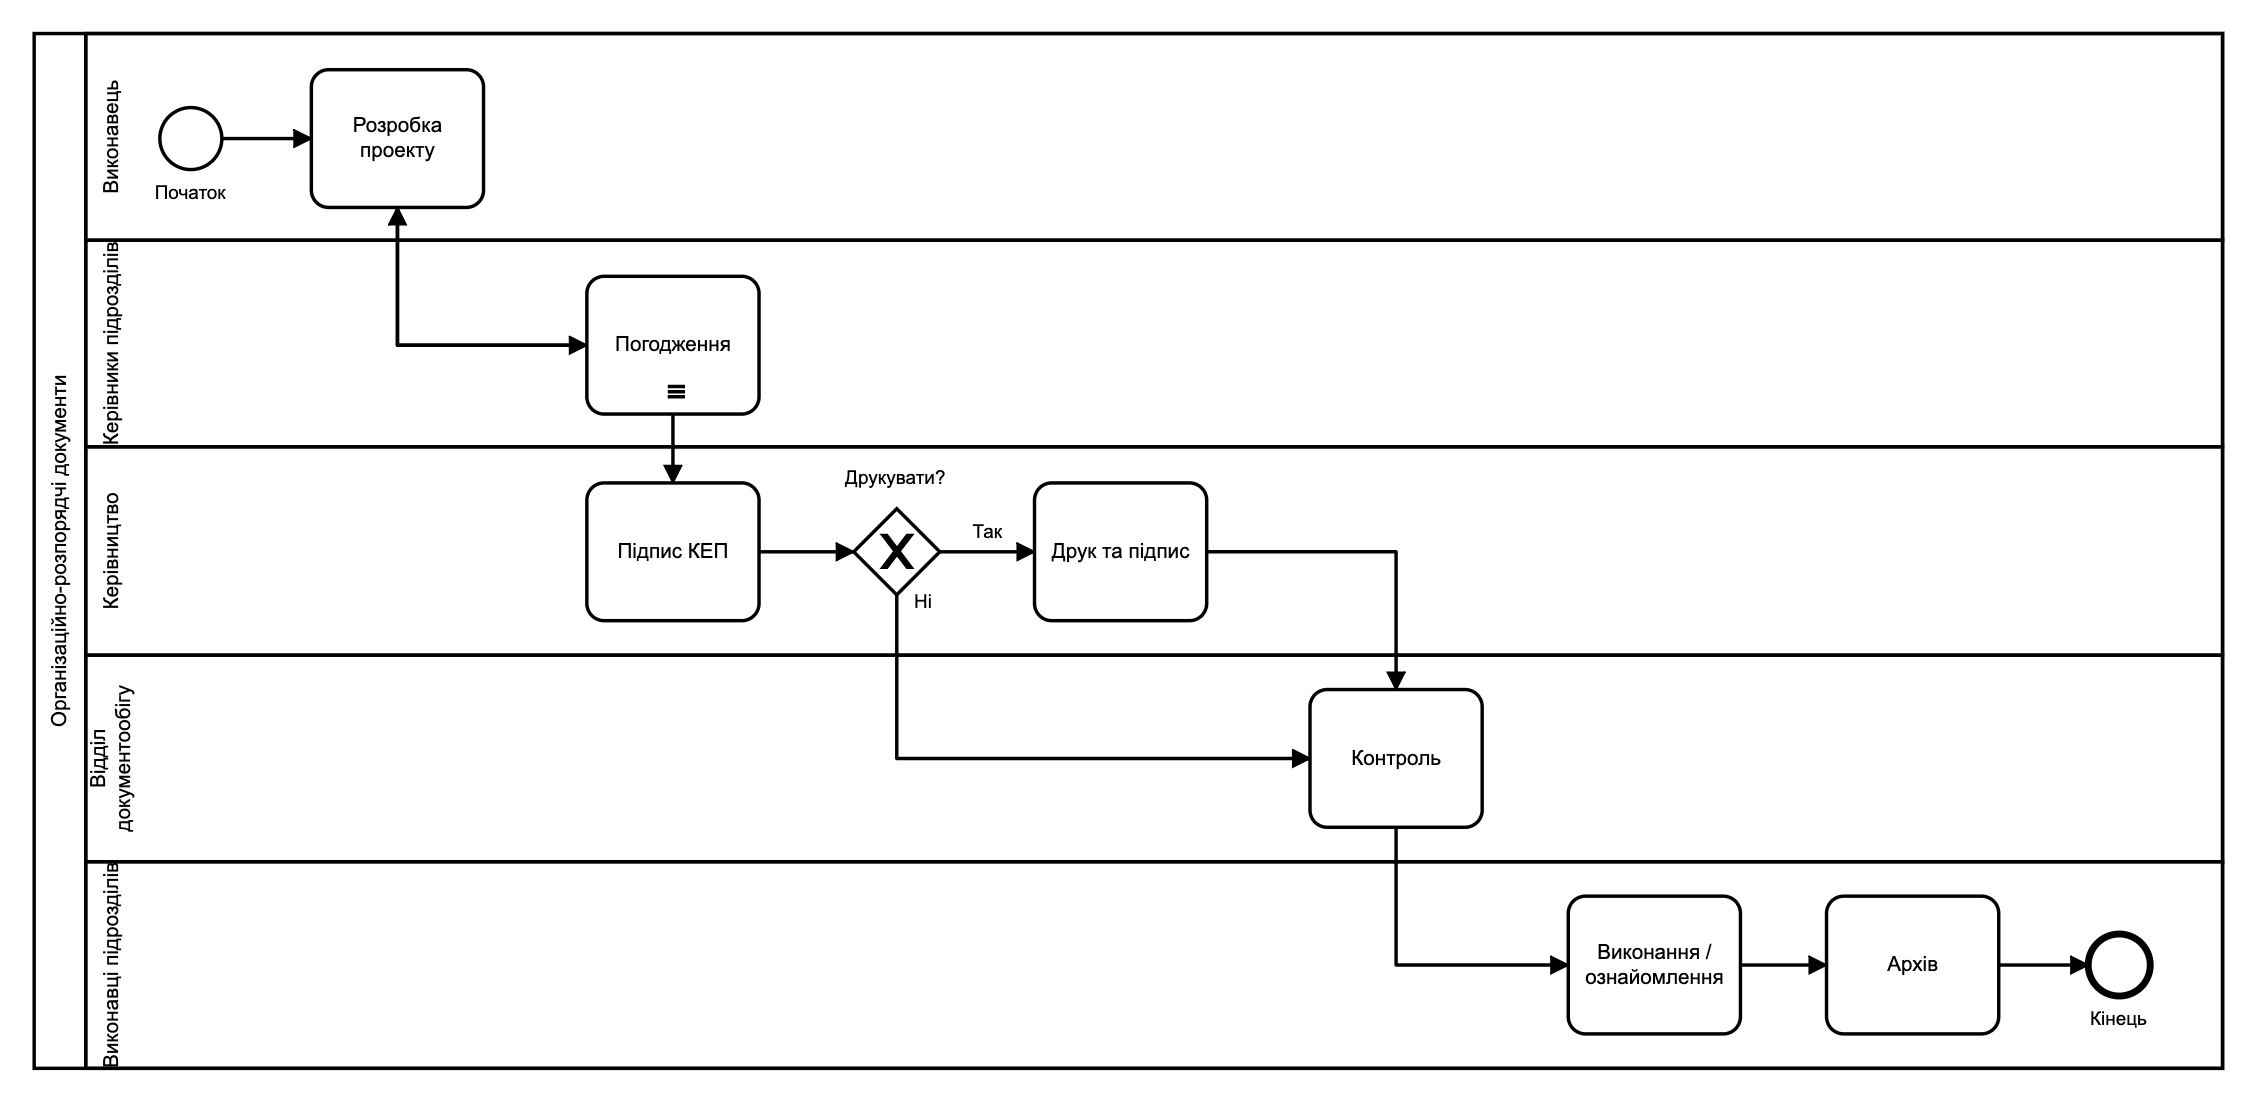
\includegraphics[scale=0.25]{orgDoc.png}}
\caption{Бізнес-процес просування організаційно-розпорядчих документів}
\end{figure}

\subsubsection*{Розробка проєкту документа}

На цьому початковому етапі розробляється базовий електронний проєкт документа. Спочатку уважно заповнюються всі необхідні мета-реквізити в електронній картці документа; після її збереження до картки автоматично прикріплюється візуальний шаблон документа, який відіграватиме роль оригіналу. Далі виконавець вносить безпосередній змістовий вміст документа в цей оригінал і зберігає його версію. Ініціатор у системі додає всіх виконавців, кому адресований майбутній наказ. Варто зазначити, що використовуючи поле «Адресовано», система автоматично згенерує та призначить задачі відповідним виконавцям. Тільки після цих процедур документ слід передати на наступний крок.

\subsubsection*{Погодження (візування)}

На даному кроці у суворій послідовності виконується фахове погодження документа усіма особами, які були заздалегідь вказані виконавцем під час створення проєкту. Обов'язковою умовою автоматичної передачі документа на наступний етап є отримання позитивного погодження (візи) від \textbf{УСІХ} погоджуючих осіб. В іншому разі просунути документ за маршрутом далі просто неможливо. Якщо принаймні один з візуючих відхилив документ (при цьому він зобов'язаний внести обґрунтований коментар із причинами відхилення і зауваженнями до тексту чи суті наказу) — система повертає документ на першу стадію, інформуючи виконавця про необхідність його доопрацювання. Якщо ж усі без винятку особи погодили проєкт, система автоматично переводить його на наступну стадію. Після остаточного візування є можливість згенерувати та вивантажити офіційний «Аркуш погодження» у вигляді друкованої форми.

\subsubsection*{Застосування КЕП (кваліфікованого електронного підпису)}

На цій критичній стадії документ остаточно підписується в електронному вигляді уповноваженим керівництвом Міністерства. Саме в момент накладання валідного криптографічного КЕП документу присвоюється постійний інвентарний реєстраційний номер. У разі налаштування Системи електронного діловодства (СЕД) на використання візуального QR-коду, він генерується з розмірами 21 на 21 мм і надійно розміщується в нижньому лівому куті першої сторінки документа. Якщо ж політикою СЕД передбачено використання класичного лінійного штрихкоду, його алгоритмічно розміщують у правому кутку нижнього поля першої сторінки оригінального документа.

\subsubsection*{Підпис у паперовій формі}

Після електронного підписання організаційно-розпорядчого документа, у разі суворої необхідності створення так званого «паперового оригіналу», уповноважена особа патронатної служби (помічник Міністра, заступника міністра чи державного секретаря) акуратно роздруковує документ і надає його на «мокрий» підпис безпосередньо керівнику. Якщо ж відповідний організаційно-розпорядчий документ був підписаний локальним керівником певного підрозділу, необхідний паперовий примірник, як правило, роздруковує сам виконавець.

\subsubsection*{Постановка на контроль}

На даному етапі спеціалізований контролюючий структурний підрозділ аналізує завдання за документом і за необхідності здійснює його постановку на жорсткий контроль, вказуючи також періодичність звітування. Документи та задачі, що перебувають на контролі, завжди доступні уповноваженим особам за окремим фільтром, незалежно від поточного кроку свого опрацювання. Це дає змогу ефективно відстежувати їхній статус на будь-якій стадії життєвого циклу, чітко контролювати своєчасність виконання, проводити комплексну аналітику тощо, не втручаючись напролом в операційний перебіг.

\subsubsection*{Виконання та ознайомлення}

На даному виконавчому етапі відповідальний за ознайомлення або контроль структурний підрозділ бере до уваги директиви, викладені в документі. За всіма документами на контролі в режимі реального часу відстежується їхній актуальний статус. Працівники можуть переглядати, аналізувати та закривати задачі паралельно з тим, як потік процесів продовжує свій рух інформаційними каналами міністерства.

\subsubsection*{Цифровий шифрований архів}

Після виконання завдань та загального ознайомлення адресатів, документ офіційно переходить у довгостроковий цифровий Архів. Система архіву додатково накладає електронні підписи КЕП самого Архіву, надійно цементуючи файл. Крім того, задля гарантування непорушності, Архів навічно утримує повну криптографічну історію та ланцюг усіх застосованих проміжних сертифікатів: починаючи від локального АЦСК та закінчуючи ЦЗО.

\subsubsection{Звернення громадян}

\begin{figure}[!htbp]
\centerline{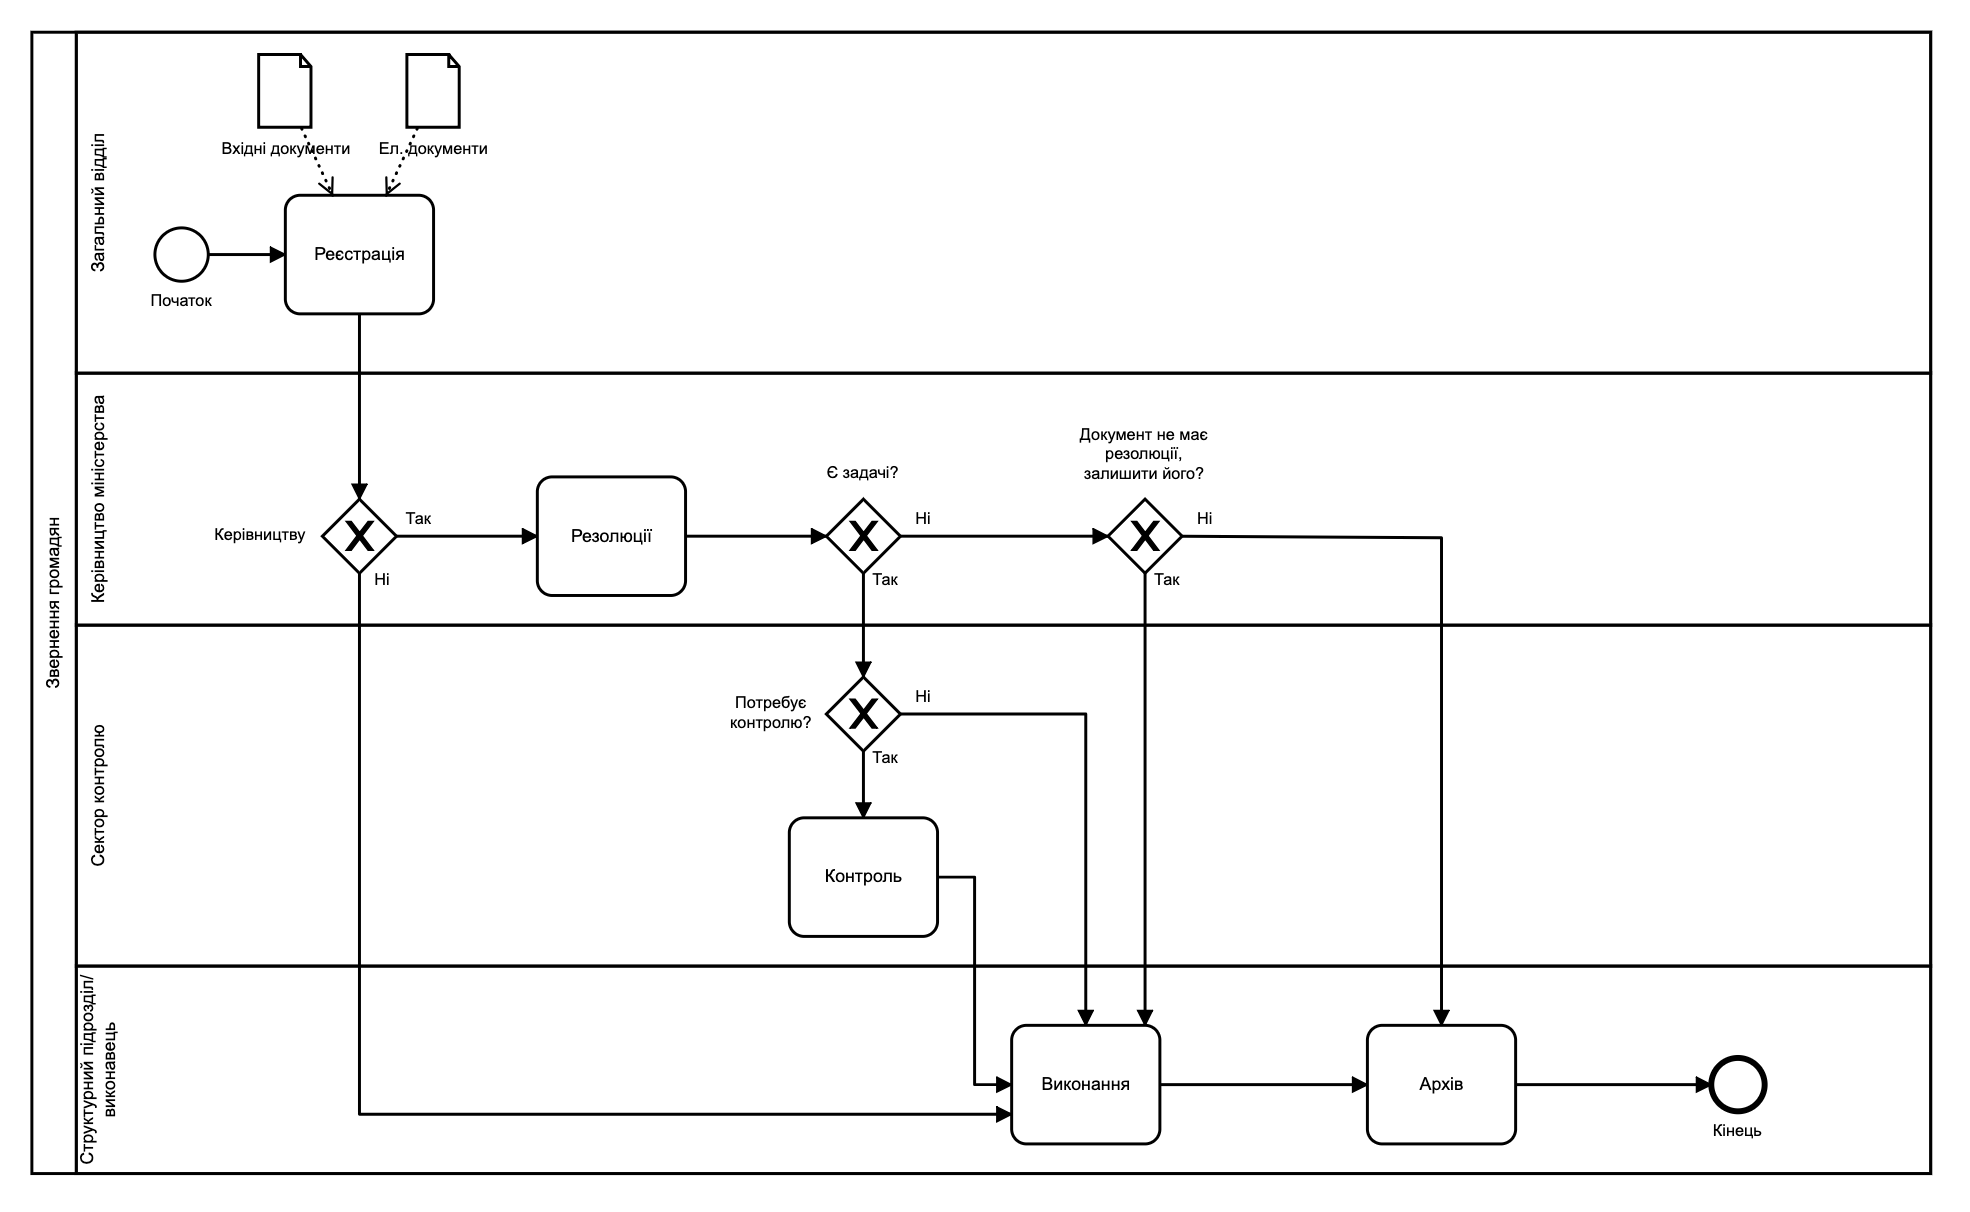
\includegraphics[scale=0.3]{citizenInquire.png}}
\caption{Бізнес-процес опрацювання звернень громадян}
\end{figure}

\newpage
\subsection{Елементи інтерфейсу}

У цьому розділі зібрано мінімально необхідну кількість бізнес-форм та UI-компонентів, розроблених спеціально для CRM-сегменту системи електронного діловодства (СЕД). Вони є індивідуальними та критично необхідними для виконання функціональних вимог, висунутих замовниками.

\subsubsection{Календар}

Базовий елемент інтерфейсу «Календар» взято з відкритої бібліотеки NITRO, проте він адаптований і потребує застосування додаткової кастомної стилізації.

\begin{figure}[!htbp]
\centerline{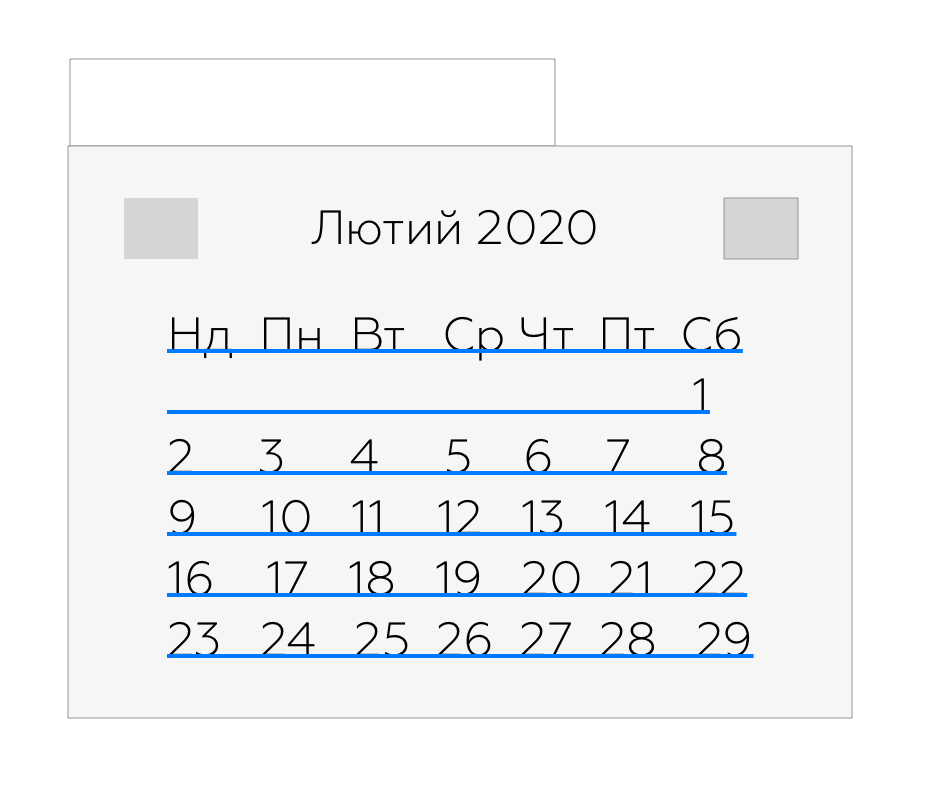
\includegraphics[scale=0.4]{calendar.png}}
\caption{Контрольний елемент «Календар»}
\end{figure}

\newpage
\subsubsection{Пошук за довільними атрибутами}

Для забезпечення швидкого та релевантного пошуку за величезними загальнонаціональними словниками та бізнес-об'єктами в системі передбачено створення спеціалізованого скалярного комбо-пошуку. Він дає змогу виконувати віддалені запити за довільними полями в централізованому сховищі даних (наприклад, виконувати миттєвий пошук за довідниками співробітників, індексами населених пунктів КОАТУУ тощо).

\begin{figure}[!htbp]
\centerline{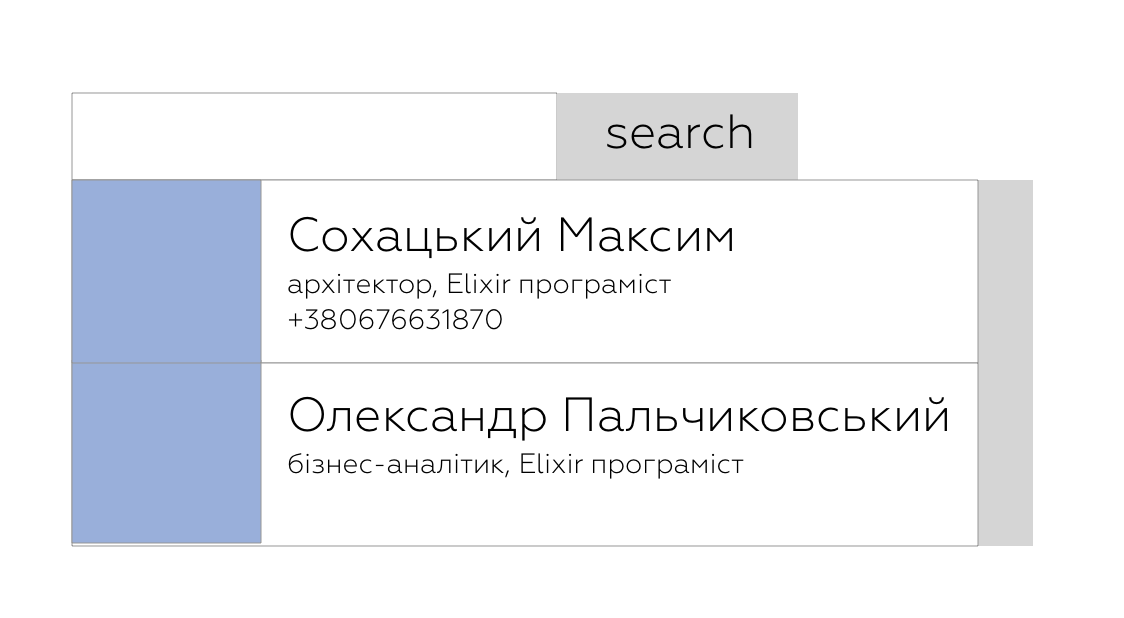
\includegraphics[scale=0.3]{comboLookup.png}}
\caption{Контрольний елемент віддаленого пошуку в базі даних}
\end{figure}

\subsubsection{Форми редагування та пошуку}

Для кожного зареєстрованого типу документа чи сутності в системі створюються дві паралельні форми: форма пошуку і форма редагування (яка одночасно виступає як форма створення нового об'єкта). Наявність цих двох різних сутностей суворо вмотивована відмінністю у логіці їхніх валідаторів. У формі пошуку валідатори апріорі повинні дозволяти залишати поля порожніми, тоді як для форми редагування валідатори зобов'язані безкомпромісно перевіряти сувору повноту та валідність заповнення полів критичних бізнес-об'єктів.

\begin{figure}[!htbp]
\centerline{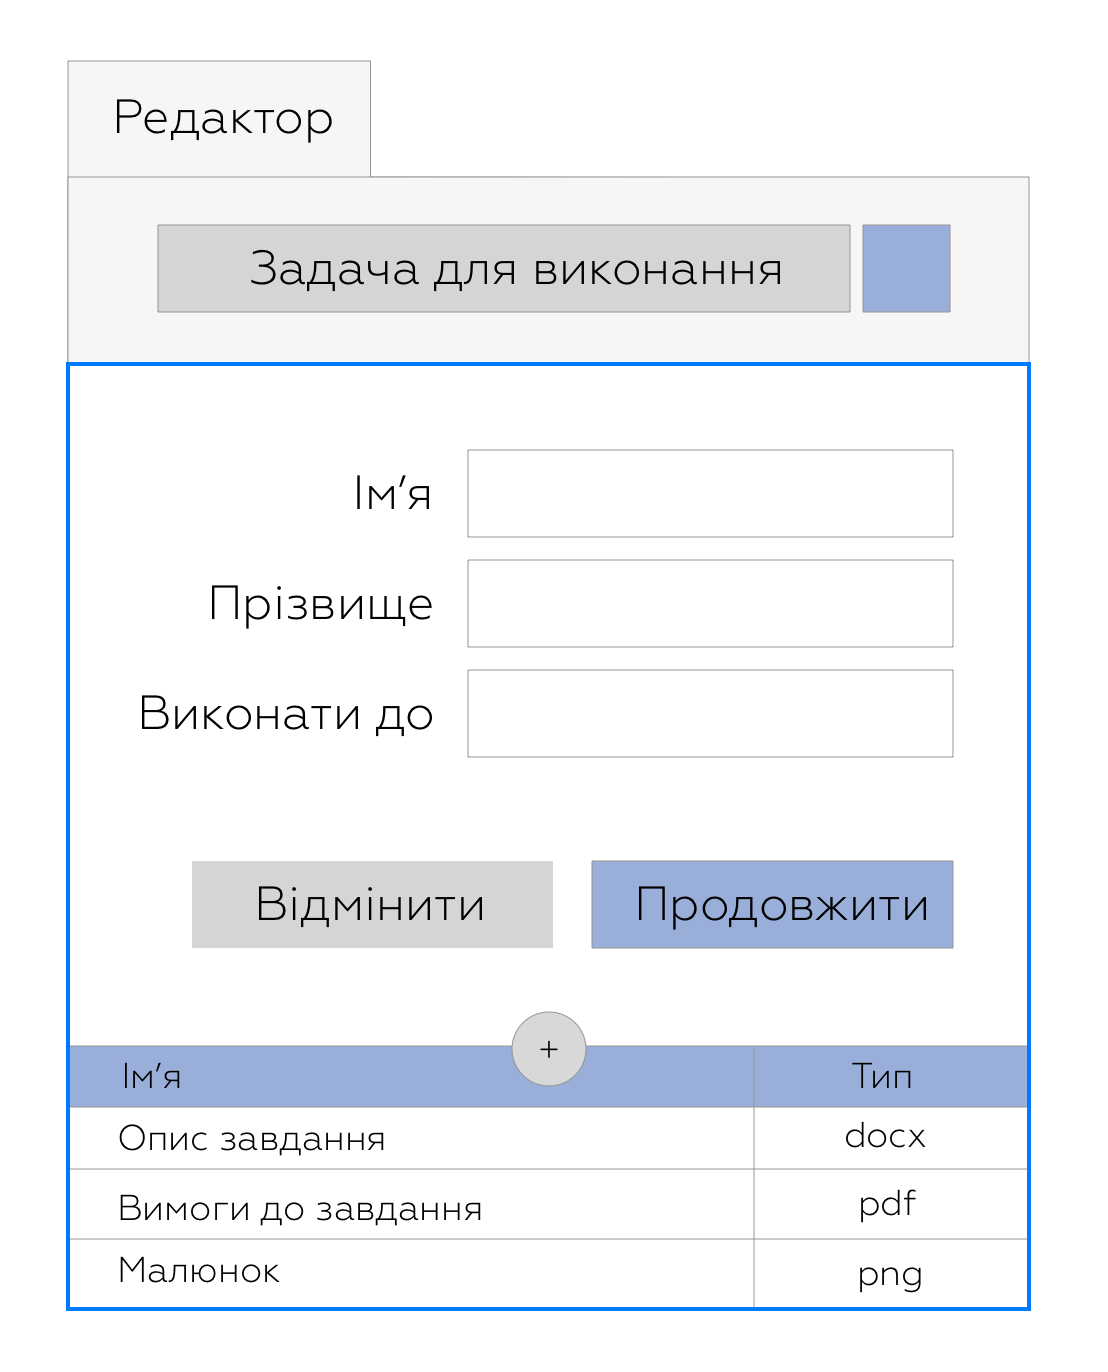
\includegraphics[scale=0.3]{editForm.png}}
\caption{Контрольний елемент інтерактивного редагування документа та прикріплених підлеглих файлів}
\end{figure}

\newpage
\subsubsection{Управління бізнес-процесом}

Для ефективного управління щоденними завданнями, миттєвого доступу до документів у розрізі певного процесу, створення дочірніх документів, а також для процесів візування, підпису або подальшої маршрутизації документів по бізнес-ланцюгах в інтерфейсі використовується стандартизований контрольний елемент управління бізнес-процесом.

\begin{figure}[!htbp]
\centerline{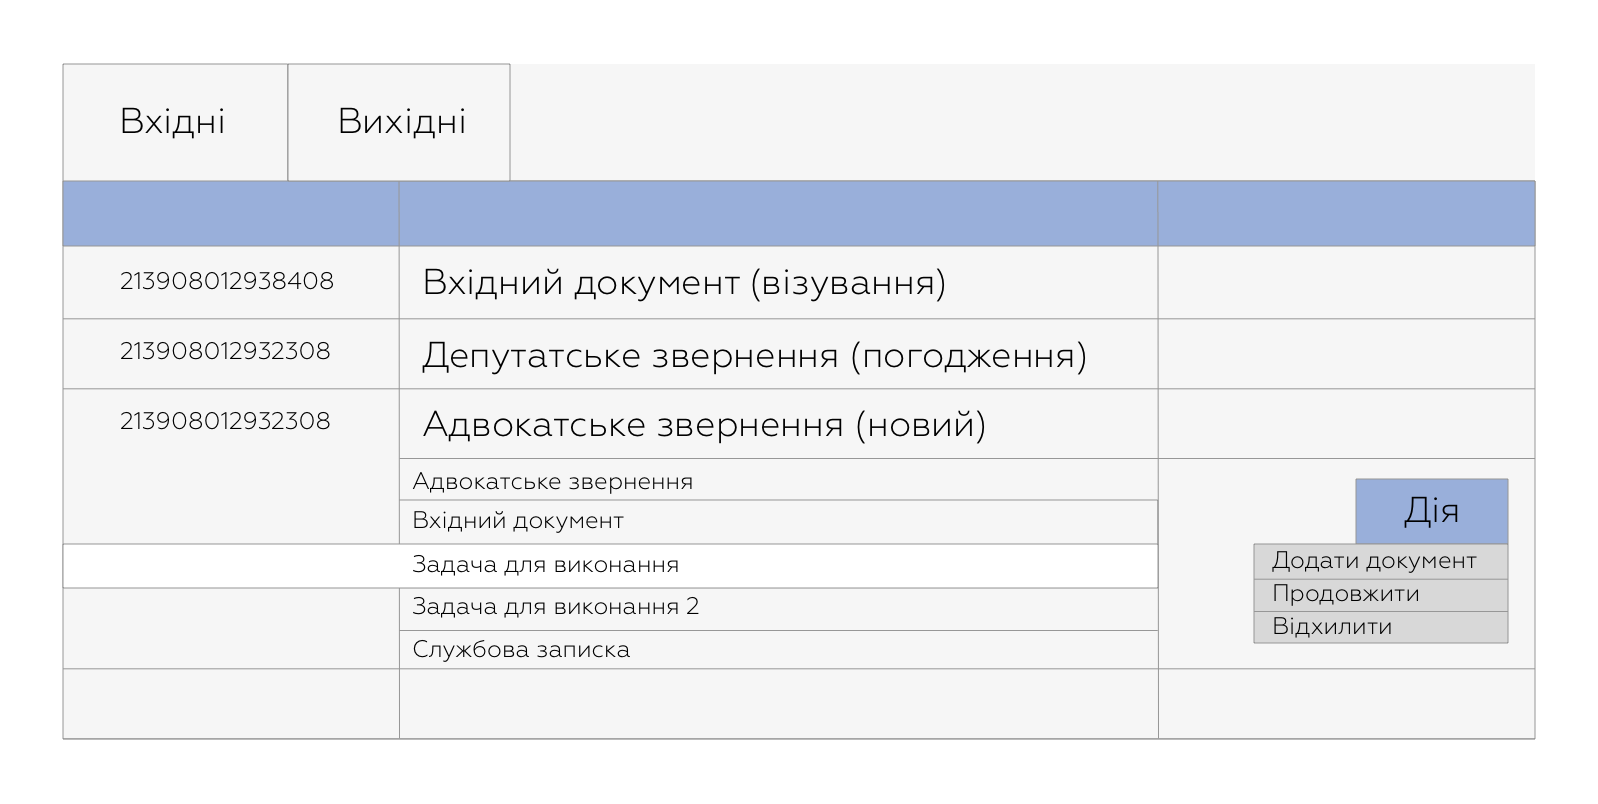
\includegraphics[scale=0.3]{bpeControl.png}}
\caption{Контрольний елемент управління бізнес-процесами}
\end{figure}

\subsubsection{Документи у виконавчих процесах}

Під час навігації сторінками та документами окремого процесу інтерфейс гарантує миттєве відображення вмісту будь-якого підлеглого документа у спеціальній лівій робочій панелі головної сторінки користувача, що значно прискорює аналіз та прийняття рішень.

\begin{figure}[!htbp]
\centerline{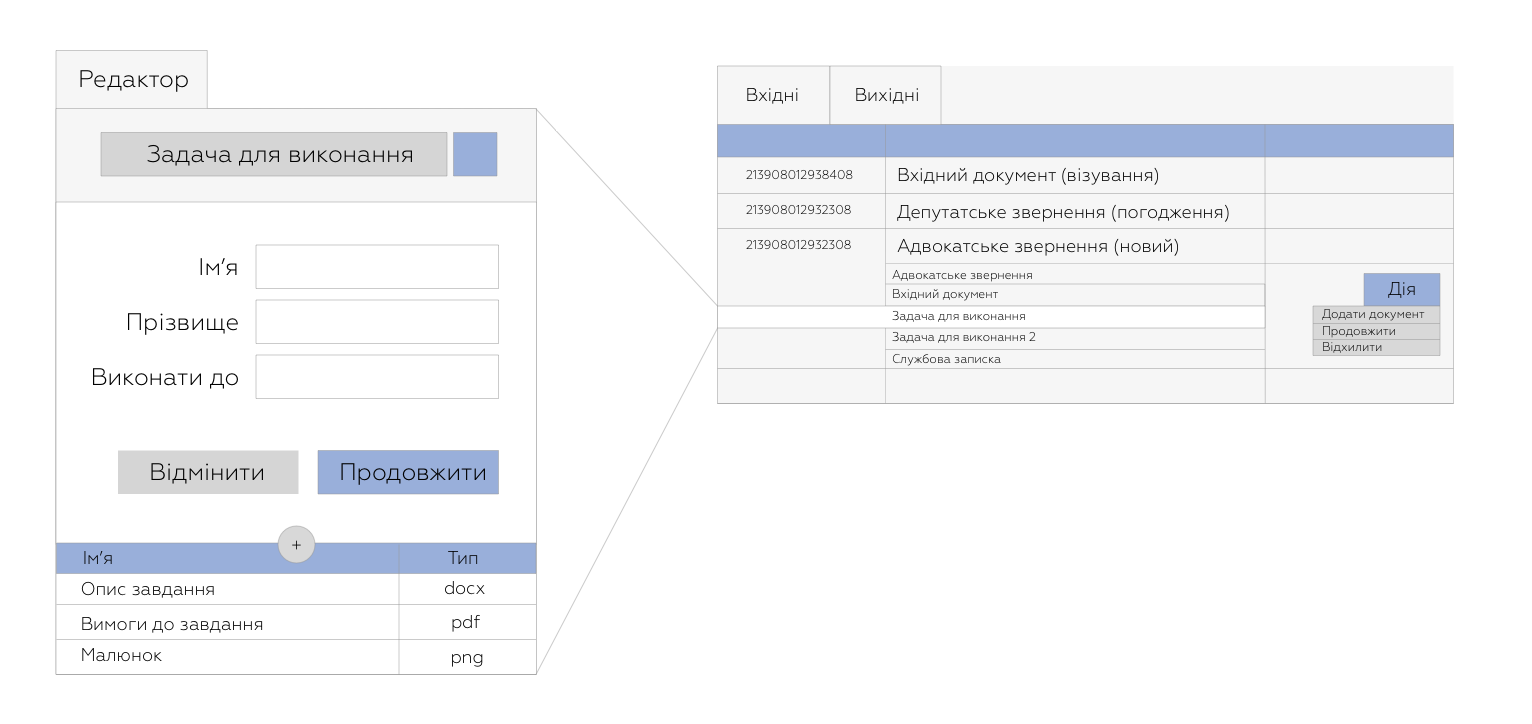
\includegraphics[scale=0.4]{searchBpe.png}}
\caption{Інструменти навігації за документами обраного бізнес-процесу}
\end{figure}

\newpage
\subsubsection{Використання вбудованих контролів у формах}

Приклад практичного використання універсального контрольного елемента довільного пошуку-комболукапу всередині складних комплексних форм.

\begin{figure}[!htbp]
\centerline{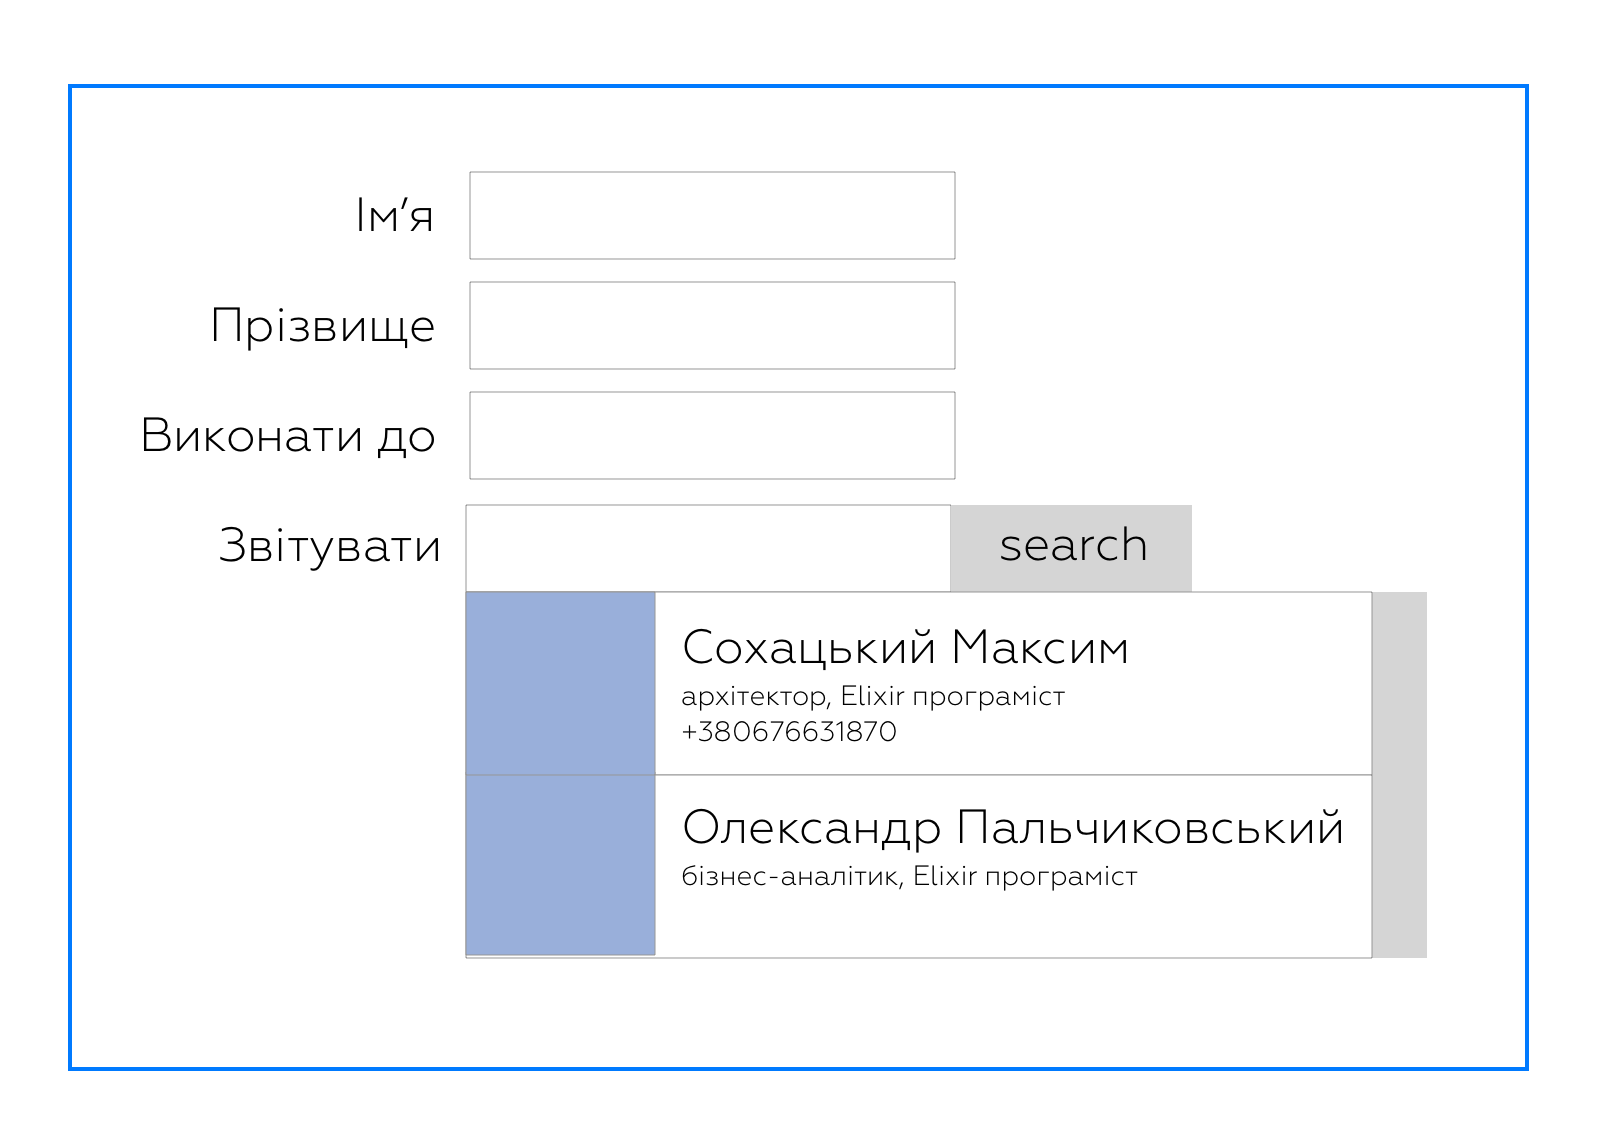
\includegraphics[scale=0.3]{comboLookupForm.png}}
\caption{Приклад безшовної інтеграції контрольних елементів у структурованих формах}
\end{figure}

\subsubsection{Контрольний елемент КОАТУУ}

Наочний приклад роботи спеціалізованого державного контрольного елемента пошуку за класифікатором КОАТУУ.

\begin{figure}[!htbp]
\centerline{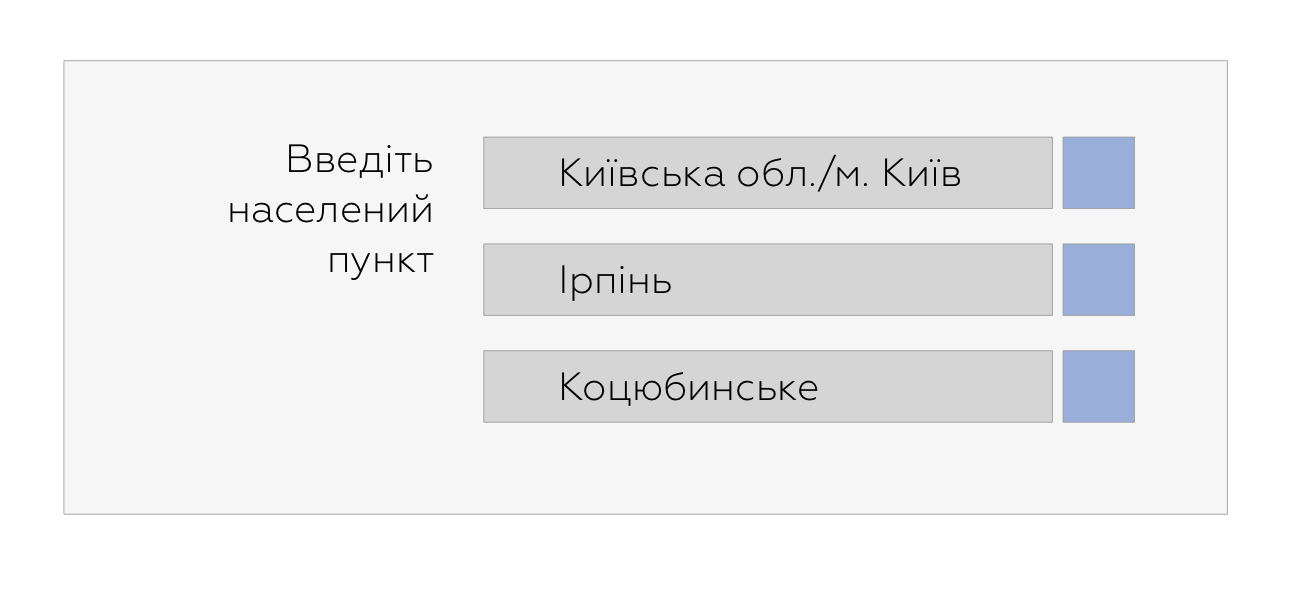
\includegraphics[scale=0.3]{koatuu.png}}
\caption{Приклад спеціалізованого використання контрольного елемента КОАТУУ}
\end{figure}

\newpage
\subsection{Редактори та додатки}

Тут перелічено контролери основних сторінок, кожна з яких є повноцінним незалежним SPA (Single Page Application) вебдодатком, завантаженим в екосистему.

\subsubsection{Вхід до системи}

Головна сторінка входу та первинної авторизації користувачів з використанням ЕЦП (КЕП).

\begin{figure}[!htbp]
\centerline{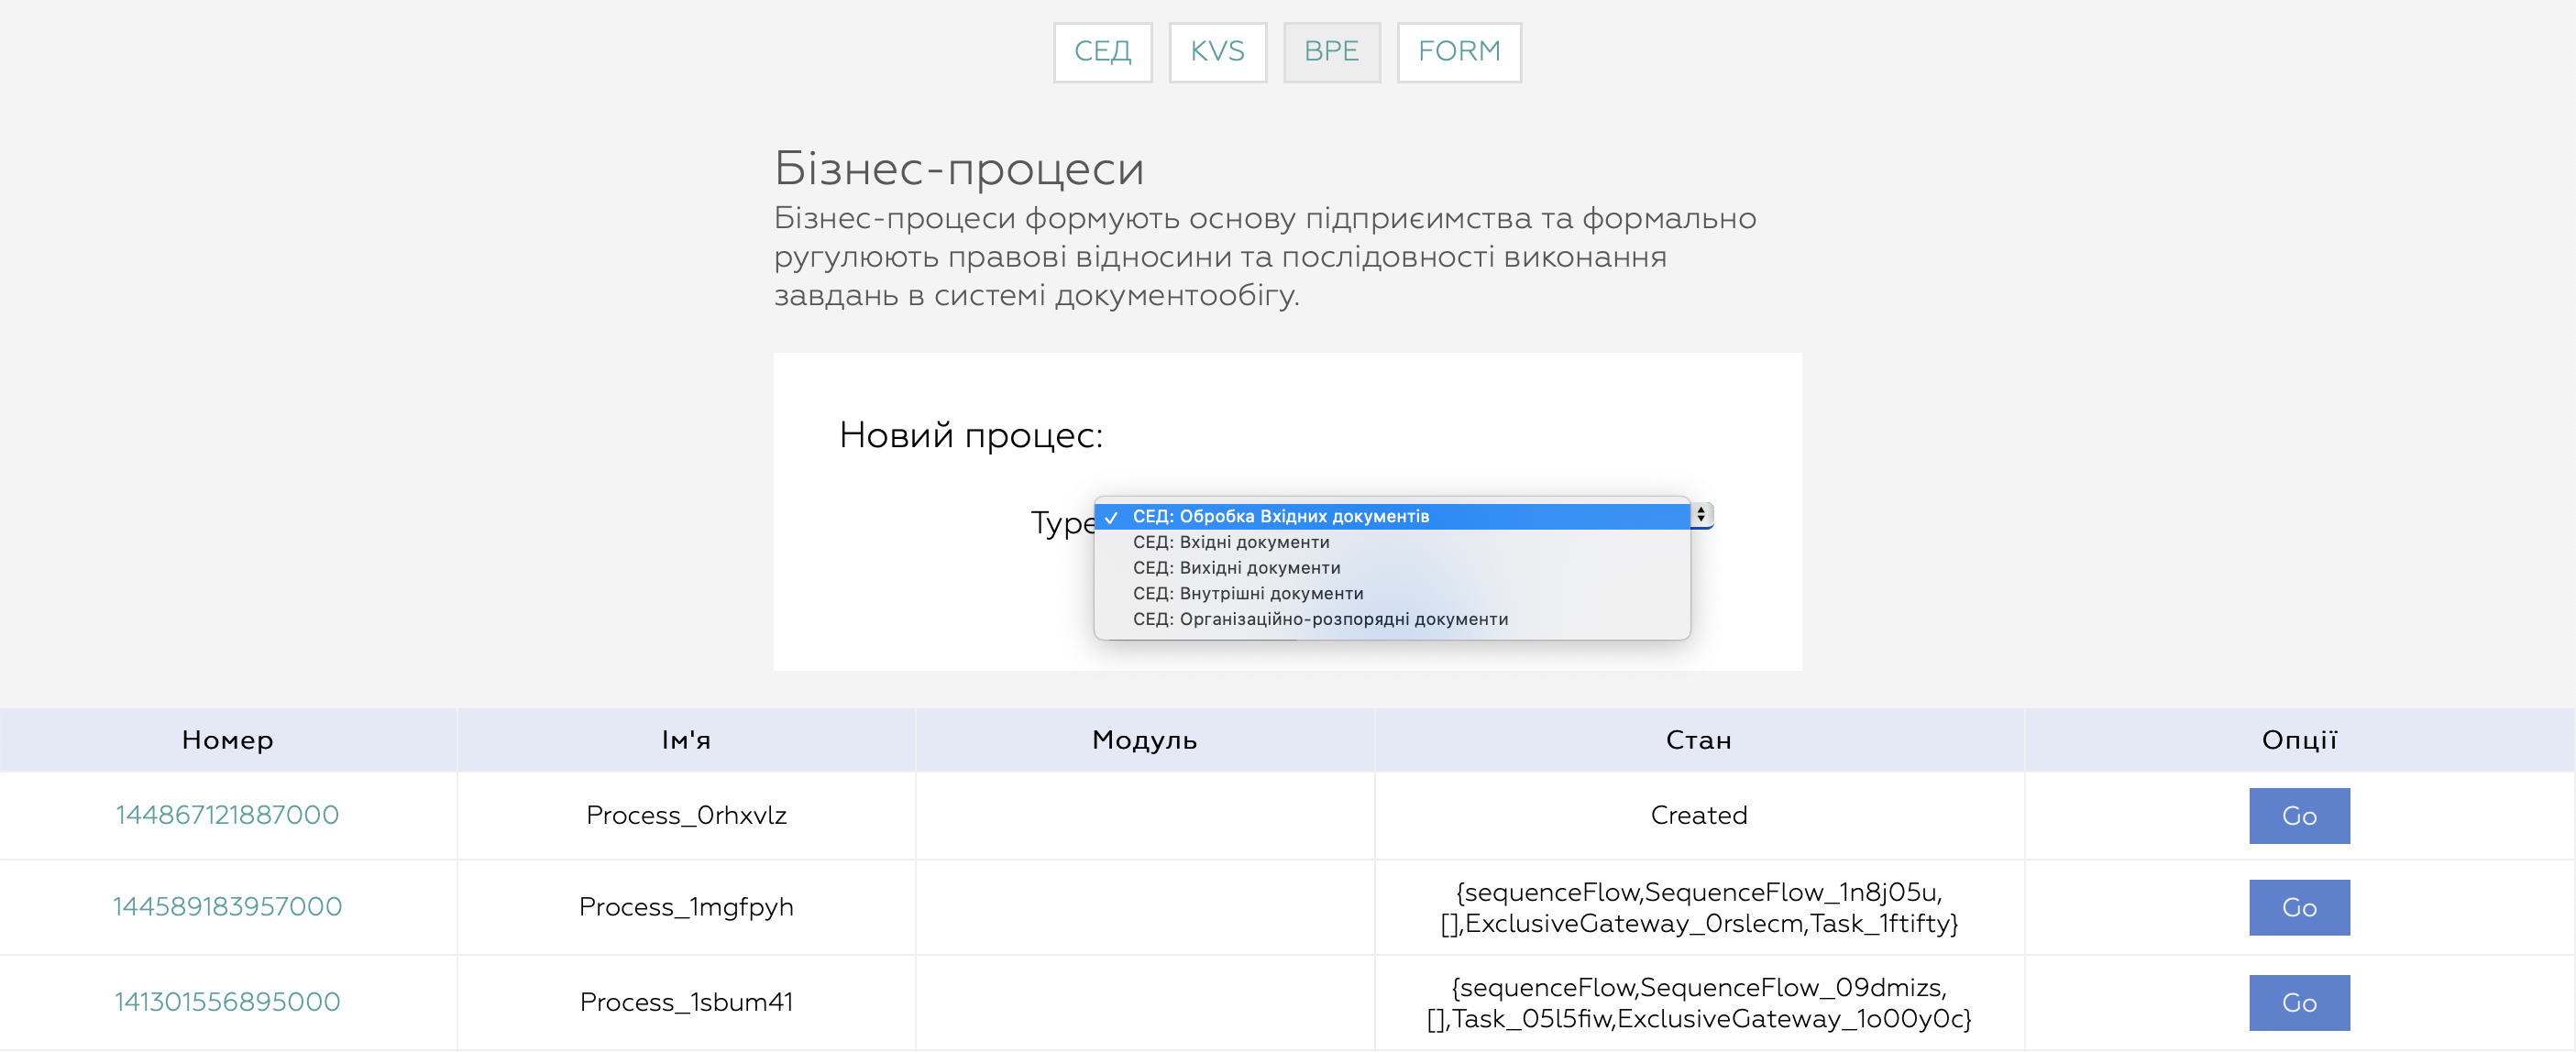
\includegraphics[scale=0.4]{ldap.png}}
\caption{Захищена сторінка входу в систему}
\end{figure}

\newpage
\subsubsection{Робота з документами}

Основна консоль системи та найголовніша робоча сторінка користувача, яка слугує хабом для безпосередньої обробки документів у робочих бізнес-процесах.

\begin{figure}[!htbp]
\centerline{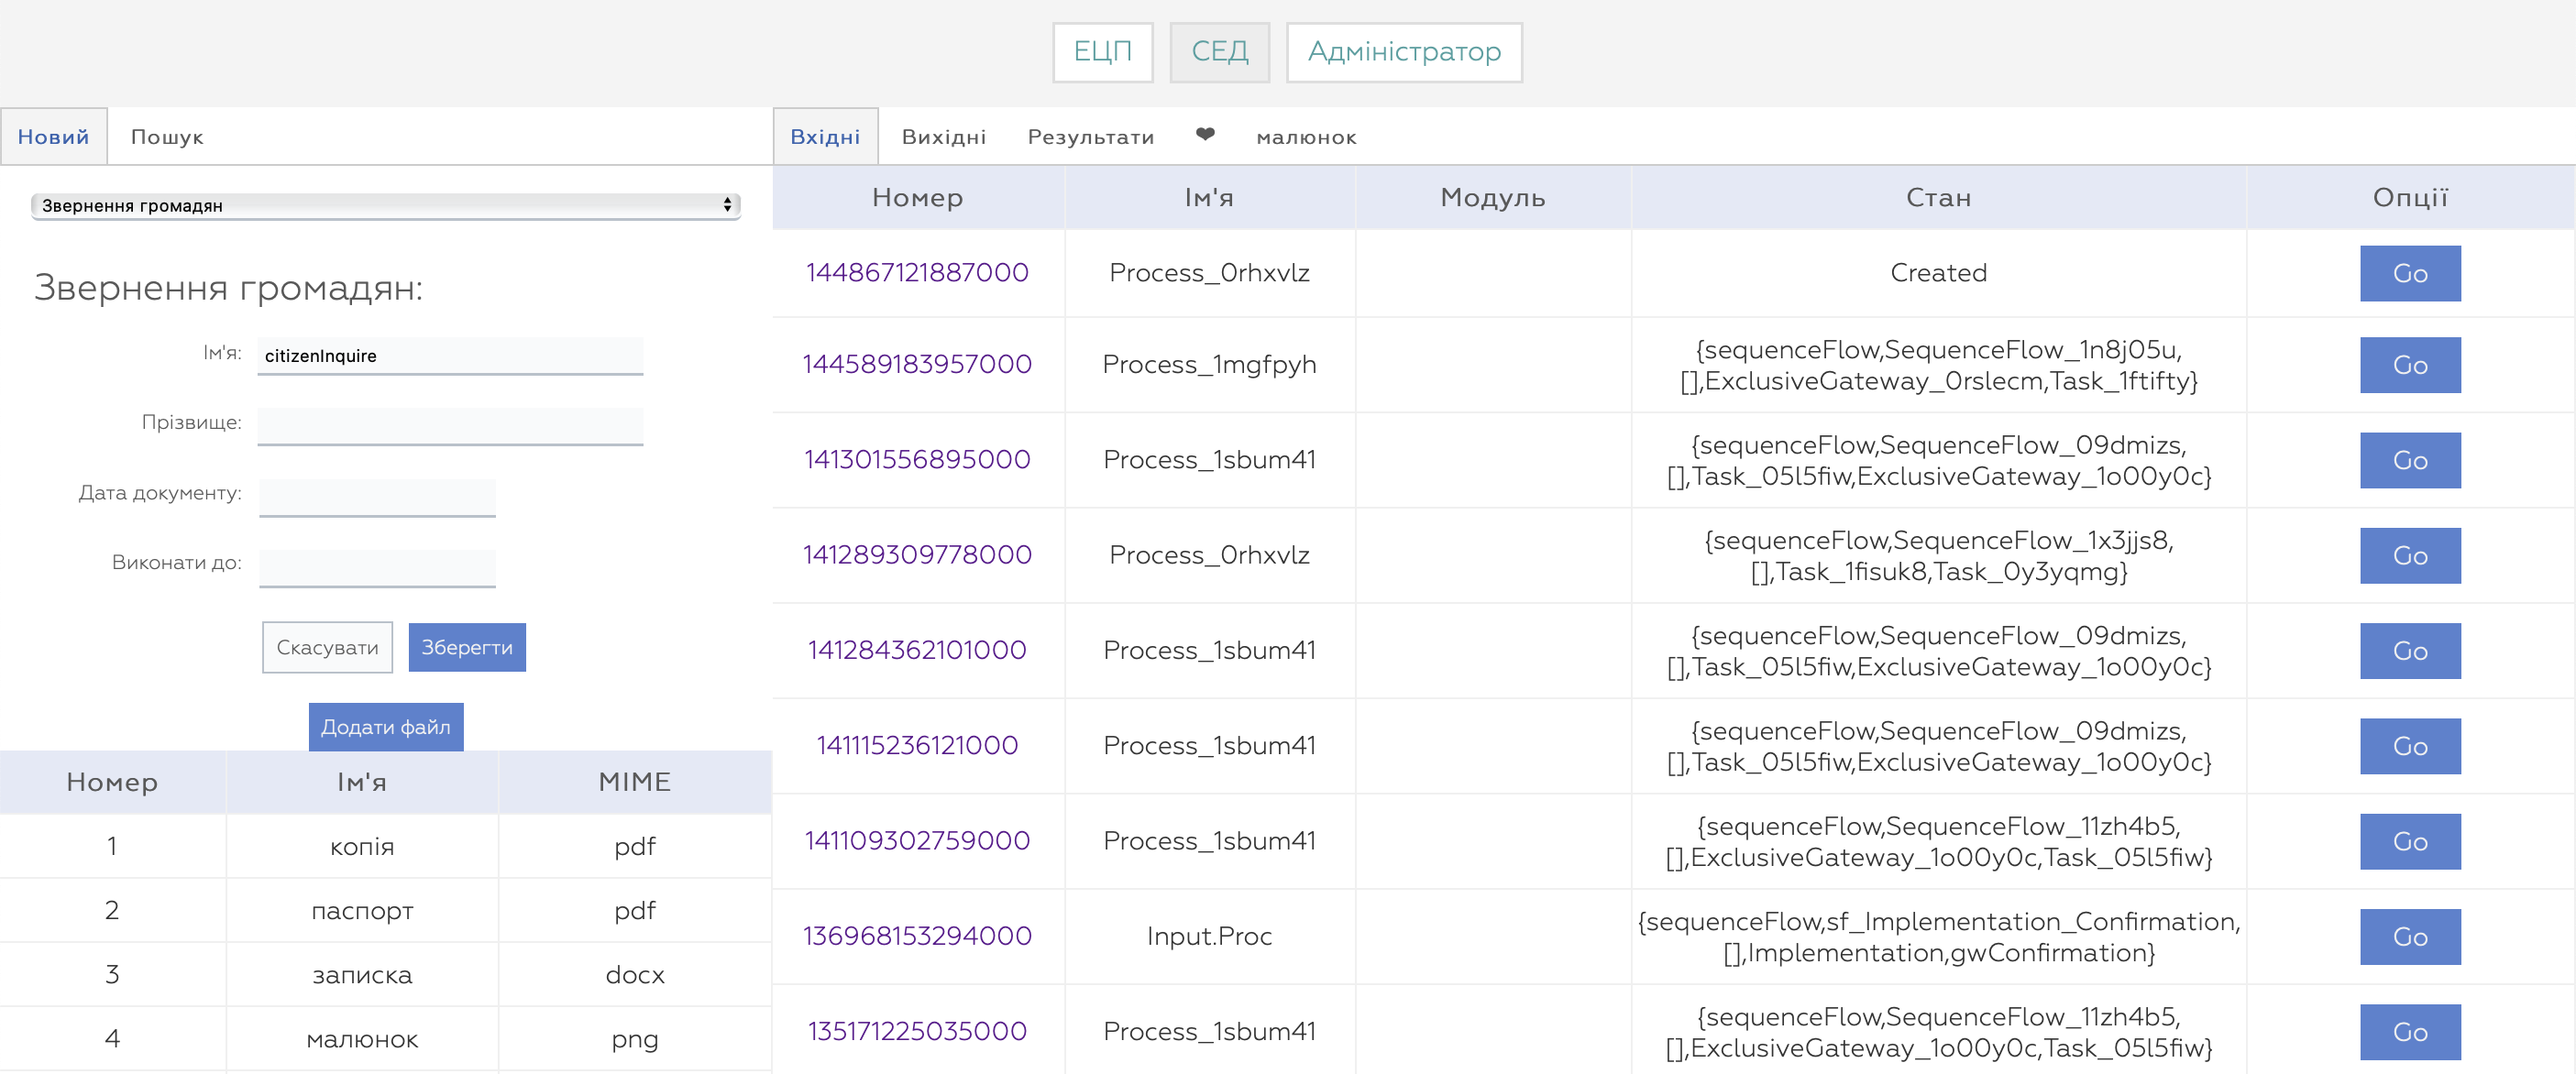
\includegraphics[scale=0.2]{crm.png}}
\caption{Функціональна сторінка роботи зі вхідними та вихідними документами}
\end{figure}

При навігації за документами процесу користувачеві доступне миттєве відображення змісту підлеглого документа або його вкладень на лівій інформаційній панелі головної сторінки, що оптимізує час опрацювання.

\begin{figure}[!htbp]
\centerline{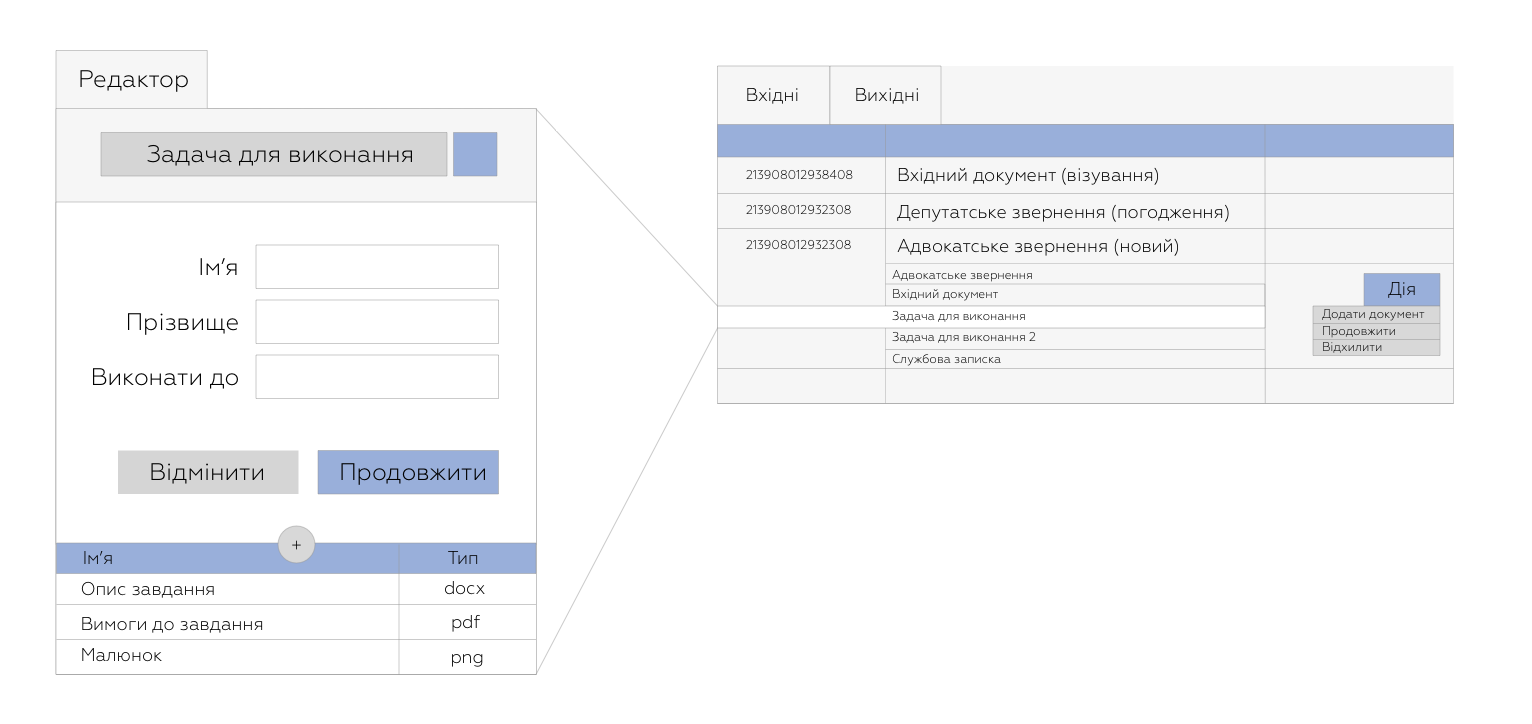
\includegraphics[scale=0.4]{searchBpe.png}}
\caption{Мініатюри та швидка навігація за підлеглими документами}
\end{figure}

\newpage
\subsection{Конструктор процесів}

Тут представлено спеціалізовані адміністративні сторінки управління системою, які призначені для системних архітекторів.

\subsubsection{Бізнес-об'єкти}

Глобальний централізований каталог усіх типів бізнес-об'єктів (документів, організацій, форм), які наразі існують у системі.

\subsubsection{Бізнес-процеси}

Вичерпний перелік усіх зареєстрованих та затверджених бізнес-процесів у системі, із забезпеченою можливістю гнучкого тестування, відлагоджування і проєктування маршрутів.

\subsubsection{Бізнес-форми}

Перелік усіх стандартизованих візуальних форм документів та кастомних бізнес-форм користувача, спеціально зареєстрованих для рендерингу в системі.

\subsection{Мова програмування FormalTalk}
